\chapter{Methodology}\label{Ch:Methodology}
This chapter describes the project workflow, beginning with the generation of 3D synthetic datasets used for training, validating, and testing the models (Section~\ref{Sec:data_gen}). Section~\ref{Subsec:Fluvgan} details the \gls{gan} framework, including the network architectures, the facies representation strategy, and the loss functions employed during training. Finally, Section~\ref{Sec:eval} introduces the metrics and simulation methods used to evaluate the geological realism and practical utility of the generated realizations.
%=====================================================================================%
\section{Dataset Generation}\label{Sec:data_gen}
In order to test the applicability of \glspl{gan} several new datasets had to be generated. Training deep learning algorithms for 3D geomodelling requires a substantial volume of high-fidelity training data. The new datasets were generated using FLUMY~\parencite{martin-hal-01313232}, a process-based stochastic modelling software designed to reproduce meandering channelized reservoirs. Based on sedimentological rules, the software reproduces facies type, grain size and deposition time for each voxel in th 3D volume.
%=====================================================================================%
\subsection{Dataset Descriptions}\label{Subsec:Dataset_descriptions}
To test the \gls{gan} in different scenario', three distinct geological conceptual models were curated to capture a range of environments for the Delft Sandstone reservoir. The setting specific input parameters are shown in Table \ref{tab:NEXUS_input}.
\begin{table}[htbp]
    \centering
    \renewcommand{\arraystretch}{1.2}
    \begin{tabular}{p{0.40\textwidth}ccc}
        \hline
        \textbf{Parameter} & \textbf{Setting 1} & \textbf{Setting 2} & \textbf{Setting 3} \\
        \hline
        Net-to-Gross (\%) & 67 & 67 & 67 \\
        Max. Channel Depth (m) & 5 & 6 & 7 \\
        Max. Sand Body Extension & 80 & 100 & 120 \\
        \hline
    \end{tabular}
    \caption{NEXUS input parameters for the three training datasets. }
    \label{tab:NEXUS_input}
\end{table}
The hypothesized depositional environments are split across three discrete suites, Ranging from a Lower plain to Upper plain deltaic characteristics in terms of increasing channel depth and wider sand bodies. Beyond these constraints, all generated models share a uniform reservoir scale with a total grid resolution fixed at 32x128×128 voxels. In order to allow for well placement in the samples, the final dimension should encompass an area of at least 2000x2000m as the \textbf{DEL-GT-01} and \textbf{DEL-GT-02-S2} have an 1500m spacing between them. Establishing this specific grid resolution combined with a standard voxel dimension of 20 m×20 m×1 m means that the total simulated domain covers a volume of 2560 m×2560 m×32 m. Every single voxel within this acute 32~m vertical interval is ultimately encoded with 1 of the 14 distinct facies (see \ref{tab:facies_config_overview}) available in FLUMY, of which only 9 facies actually occured in the sample ensemble due to the settings specific parameters.

\subsection{Sample preprocessing}
To comprehensively assess the capabilities of \glspl{gan}, the synthetic training datasets are prepared at two distinct categorical resolutions. These two distinct resolutions consist of a high-fidelity 9-facies dataset and an upscaled 3-facies dataset. The high-fidelity 9-facies dataset preserves the detailed depositional environments generated by FLUMY, serving as a baseline to evaluate the model's pure generative capacity and its ability to replicate highly complex spatial distributions. While evaluating this generative capacity is crucial, practical field application requires conditioning the model to actual subsurface observations. These actual subsurface observations, derived from the cored section of the \textbf{DEL-GT-01} well, are strictly classified into three primary facies associations (Section \ref{subsec:geology_DGR}). Because the hard well data only resolves to three distinct associations, the original FLUMY depositional environments must be grouped accordingly to create the upscaled 3-facies dataset. This grouping process aggregates the detailed environments into broader categories, as detailed in Table \ref{tab:3_facies_grouping}.

\begin{table}[htbp]
    \centering
    \renewcommand{\arraystretch}{1.4}
    \begin{tabular}{c p{0.30\textwidth} l p{0.40\textwidth}}
        \hline
        \textbf{Value} & \textbf{Facies Key} & \textbf{Color} & \textbf{Description} \\
        \hline
        1 & Channel \& Point Bar (FA1) & \textcolor[HTML]{F3DD12}{\rule{10pt}{10pt}} & Grouped proximal deposits: Channel Lag (1), Point Bar (2), Sand Plug (3), and Crevasse Splay I (4). \\
        2 & Levee \& Crevasse (FA2) & \textcolor[HTML]{27AE60}{\rule{10pt}{10pt}} & Grouped intermediate deposits: Crevasse Channel (5), Crevasse Splay II (6), and Levee (7). \\
        3 & Overbank Fines (FA3) & \textcolor[HTML]{33FF00}{\rule{10pt}{10pt}} & Grouped distal deposits: Overbank (8), Mud Plug (9), Hemipelagic Plug (10), Wetland/Paleosol (11), Draping (12), and Pelagic (13). \\
        \hline
    \end{tabular}
    \caption{Overview of the upscaled 3-facies grouping used for the generative modelling, aggregated from the original 13 FLUMY depositional environments (See Table \ref{tab:facies_config_overview} for the original facies).}
    \label{tab:3_facies_grouping}
\end{table}

Beyond this grouping process, the categorical nature of both the 3-facies and 9-facies datasets necessitates a final preprocessing step known as one-hot encoding~\parencite{goodfellow-et-al-2016}. One-hot encoding is critical because standard neural networks process continuous numerical gradients and might otherwise incorrectly interpret integer facies labels as having an ordinal, mathematical relationship. This ordinal misinterpretation is prevented by transforming the original 3D volume into an expanded 4D tensor, where class is assigned its own dedicated spatial channel. Each spatial channel indicates the presence or absence of a specific facies using values of 1 and -1 (Read more on one-hot encoding appendix in~\ref{Appendix:One_Hot_Encoding}).

\section{Fluvgan Framework}\label{Subsec:Fluvgan}
\subsection{Model Architecture}\label{Subsec:Model_architecture}
The GAN architecture used in this project is based on the \gls{fluvgan} model, introduced by~\textcite{rongier2025afluvgan}. Thie architecture adapts the BigGAN framework~\parencite{brock2018large} to manage the complex connectivity and high resolution necessary for realistic reservoir models. Where \textcite{rongier2025atowards} used a 2-channel approach for their model, one for grain size and one for deposition time, the model used in this project comprises of either 3 or 9 channels, where each channel represents another facies based on the one-hot encoding strategy. 

The dynamic channel depth is accommodated by an architecture comprising a Generator ($\mathbf{G}$) and a Discriminator ($\mathbf{D}$) built with 3D Residual blocks. These blocks enable the generator to transform a, in this case, 100-dimensional latent vector $\mathbf{z^{*}}$ into a $C \times 32 \times 128 \times 128$ volume. This volume begins as a $512 \times 4 \times 4 \times 4$ feature map, created via a 3D transposed convolution, and is then expanded by five residual upscaling blocks. The final spatial resolution is processed through a Tanh activation, ensuring the $C$ facies channels are scaled scaled from -1 to 1. Finally, an argmax function scales the one hot encoded tensor back to integers, ensuring that a 32x128x128 volume inhabited by class numbers remains. Every generated voxel is then evaluated by the discriminator, acting as a binary classifier to reduce the $C \times 32 \times 128 \times 128$ input to a single scalar logit. This logit is produced through five residual downscaling blocks that iteratively reduce spatial resolution while increasing the channel count to 512. A simpel visual representation of the model can be seen in figure~\ref{fig:fluvgan_architecture}. In total, the generator involves roughly 11.6 million trainable parameters while the discriminator has about 2.0 million trainable parameters.

\begin{figure}[t]
    \centering
    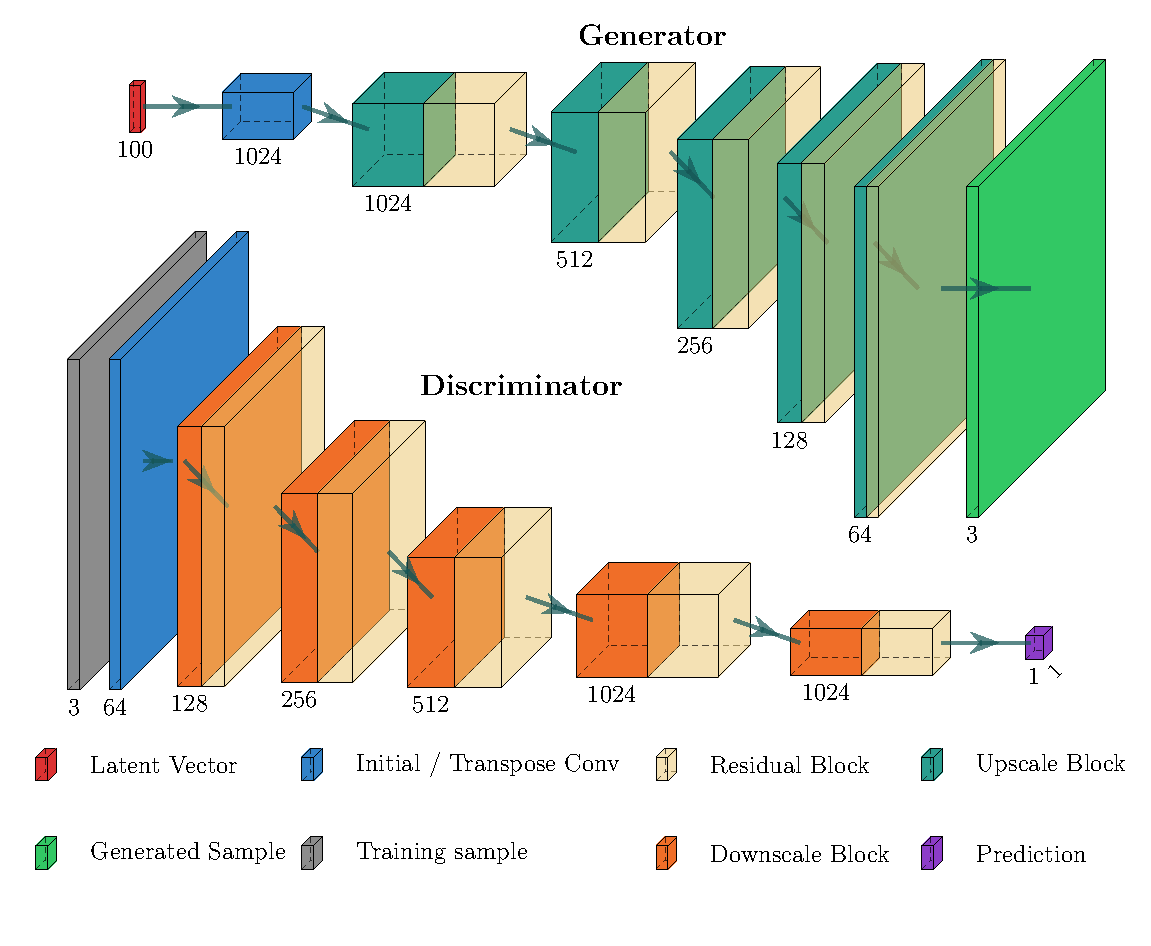
\includegraphics[width=0.9\textwidth]{figures/methodology/Architecture/FluvGan.pdf}
    \caption{\textbf{Top)} The Generator initiates from a 100-dimensional latent vector and expands spatial volume through successive upscale and residual blocks. During this process, feature channel density is progressively reduced from 1024 down to 3 channels to construct the final generated volume. \textbf{Bottom)} The Discriminator mirrors this pathway by receiving a 3-channel sample (training or generated) and contracting spatial dimensions through downscale blocks. To retain high-level structural patterns during downsampling, feature channels are steadily increased from 3 up to 1024 before compressing into a single purple block representing the final prediction scalar.}
    \label{fig:fluvgan_architecture}
\end{figure}

Evaluating the generated realizations begins by analyzing the foundational mathematical metrics, specifically Binary Cross-Entropy (BCE). BCE is deployed because the generator processes one-hot encoded facies, effectively turning the spatial generation into a~\textit{multi-channel binary classification task}. This classification task relies on BCE to penalize pixel-wise deviations between the generated probabilities ($\hat{y}_i$) and the true categorical labels ($y_i$), defined mathematically across $N$ voxels as:

$$ \mathcal{L}_{BCE} = - \frac{1}{N} \sum_{i=1}^N \left[ y_i \log(\hat{y}_i) + (1 - y_i) \log(1 - \hat{y}_i) \right] $$

During adversarial training, instability often manifests as exploding logarithmic losses when either the Generator $\mathbf{G}$ or Discriminator $\mathbf{D}$ becomes too confident in its predictions. Furthermore, poorly calibrated networks are highly susceptible to severe mode collapse, where the generator's stochastic capability is restricted. To investigate the optimal model architecture that yields stable training and diverse geological outputs, a systematic hyperparameter tuning study was conducted.

\subsubsection{Hyperparameters}
Hyperparameter tuning involves testing various combinations of network settings to evaluate their impact on model performance. The primary objective is to identify an optimal configuration that minimizes the discrepancy between the generated models and the input data, while actively preserving spatial ensemble diversity.To achieve this, baseline parameters (such as the optimizer and batch size) were kept constant (see table~\ref{tab:fixed_baseline_config}), while a specific set of architectural and training hyperparameters were varied stepwise. The complete search space for this hyperparameter study is outlined in Table~\ref{tab:Hyperparameter_search_space}.

\begin{table}[htbp!]
    \centering
    \renewcommand{\arraystretch}{1.3}
    \begin{tabular}{@{} l c p{0.45\textwidth} @{}}
        \hline
        \textbf{Hyperparameter} & \textbf{Fixed Value} & \textbf{Description} \\
        \hline
        Optimizer & Adam ($\beta_1=0, \beta_2=0.999$) & Standard optimization algorithm. \\
        Batch Size & 64 & Number of samples processed per iteration. \\
        Kernel Size & $3 \times 3 \times 3$ & Dimensions of the 3D Convolutional filters. \\
        \hline
    \end{tabular}
    \caption{Fixed baseline configurations for the Fluvgan architecture optimization study.}
    \label{tab:fixed_baseline_config}
\end{table}

\begin{table}[htbp!]
    \centering
    \renewcommand{\arraystretch}{1.3}
    \begin{tabular}{@{} l c p{0.45\textwidth} @{}}
        \hline
        \textbf{Hyperparameter} & \textbf{Search Space / Value} & \textbf{Description} \\
        \hline
        Learning Rate $\mathbf{G}$ ($\alpha_{\mathbf{G}}$) & $10^{-3}, 10^{-4}$, Dynamic & Generator step size during gradient descent. \\
        Learning Rate $\mathbf{D}$ ($\alpha_{\mathbf{D}}$) & $3\times10^{-3}, 10^{-2}$, Dynamic & Discriminator step size; testing a two-timescale update rule. \\
        num iter $\mathbf{D}$ & 1, 2 & Number of consecutive Discriminator updates per Generator update. \\
        Discriminator Penalty & None, 1, 16, 32 & Gradient penalty applied to stabilize Discriminator confidence. \\
        Double Conv Blocks & On, Off & Architectural toggle for adding secondary convolutional layers. \\
        Double ResBlocks & On, Off & Architectural toggle for adding secondary residual blocks. \\
        Training Samples & 10,000, 20,000 & Total volume of synthetic baseline data fed to the network. \\
        \hline
    \end{tabular}
    \caption{Hyperparameter search space for the Fluvgan architecture optimization study.}
    \label{tab:Hyperparameter_search_space}
\end{table}

Among the evaluated parameters, the learning rates ($\alpha_{\mathbf{G}}$ and $\alpha_{\mathbf{D}}$) along with the Discriminator update frequency (\textit{num iter} $\mathbf{D}$) are the most critical, as they directly dictate the competitive equilibrium of the adversarial minimax game. Tuning these factors enables the evaluation of the Two-Timescale Update Rule (TTUR) to maintain stable convergence and prevent mode collapse. Furthermore, the Discriminator Penalty serves as a vital regularizer to constrain gradient norms, ensuring the discriminator's confidence does not overpower the generator early in training. Lastly, the architectural toggles (Double Conv and Residual Blocks) paired with data scaling systematically isolate whether network capacity or dataset volume is primary in preserving the necessary spatial and structural diversity of the generated fluvial systems.

\subsection{Optimization \& Inversion}
While the 9-facies models are utilized to evaluate unconstrained generative performance, the 3-facies models are deployed to test practical conditioning against the \textbf{DEL-GT-01} well data. To successfully condition this generative model to real-world observations, the inversion workflow~(introduced by~\parencite{rongier2025btowards}) relies on a two-step mechanism: Latent Space Optimization and Pivotal Tuning~\parencite{roich2022pivotal}. 

First, Latent Space Optimization searches for the optimal random noise vector that best approximates the well data while keeping the pre-trained generator's weights frozen. Because this often provides a close structural approximation but rarely a perfect match, it is followed by Pivotal Tuning. This second phase uses the optimized noise vector as a static anchor and temporarily unfreezes the generator's internal weights to make microscopic adjustments. This forcefully aligns the localized output with the exact well data, while regularization prevents the collapse of broader geological realism. (A detailed mathematical formulation of this inversion process is provided in Appendix~\ref{app:optimization_math}).

\section{Evaluation Metrics}\label{Sec:eval}
Evaluating the performance of generative models on 3D spatial grids presents significant challenges, as standard metrics like Binary Cross-Entropy (BCE) or direct voxel-by-voxel assessments fail on unconditioned models. Therefore, the evaluation framework relies on metrics that capture complex geological structures and spatial uncertainty across an ensemble of generated samples.

To evaluate how closely the generated realizations resemble the training data's global morphological structures, we employ the Mean Sliced Wasserstein Distance (MSWD). Based on the optimal transport principles of the Wasserstein distance \parencite{panaretos2019statistical}, which was highlighted for geological 3D structures by \textcite{rongier2025atowards}, MSWD evaluates structural similarity without requiring rigid pixel alignment. By projecting 3D spatial distributions onto 1D linear slices and averaging the results, MSWD efficiently bypasses the computational bottleneck of high-dimensional grid volumes. It serves as our primary indicator of global architectural consistency and mode collapse during the training process. During training, the model saves 10\% of its training data exclusively for evaluation used the MSWD metric, ensuring the samples are not passed on into the Discriminator.

Beyond evaluating structural realism, quantifying the spatial uncertainty and generation diversity across the ensemble is critical. To achieve this, pixel-wise Normalized Shannon's Entropy~\parencite{shannon1948mathematical} is utilized. By calculating the entropy at each specific spatial coordinate across multiple generated models, this metric serves as a direct validation of the model's diversity. High entropy values at a given pixel indicate that the generator is capable of producing a varied distribution of facies at that location, whereas low entropy exposes areas of rigid uniformity or potential mode collapse. This pixel-wise evaluation visually maps regions of spatial conflict and agreement, which is then aggregated into a definitive scalar measure of spatial fidelity using the Jensen-Shannon (JS) divergence~\parencite{lin1991divergence}. As a symmetric metric based on Kullback-Leibler divergence~\parencite{kullback1951information}, the JS divergence measures the overall distributional disagreement between the baseline flumy and \gls{gan} models. (The full mathematical derivations for these evaluation metrics are detailed in Appendix \ref{app:evaluation_math}).

\subsubsection{Data conditioning}
While JS divergence defines the overall ensemble spread, after optimization and inversion, each individual \gls{gan} model within that ensemble must still strictly honor the physical reality at the wellbore. This physical reality at the wellbore acts as a strict spatial constraint, the localized mismatch of which is calculated using the Macro F1-score. The Macro F1-score calculates the unweighted average of the harmonic mean of precision and recall across all $C$ individual facies classes:

\[ F1_{macro} = \frac{1}{C} \sum_{c=1}^{C} \frac{2 \cdot \text{Precision}_c \cdot \text{Recall}_c}{\text{Precision}_c + \text{Recall}_c} \]

Where for each class the precision and recall scores have to calculated:

\[Precision = \frac{TP}{TP + FN}\]
\[Recall = \frac{TP}{TP + FN}\]

where true positive (TP) represents the number of correctly predicted positive pixels, false positive (FP) the predicted positive but actually negative pixels, false negative (FN) the predicted negative but actually positive pixels.

Evaluating every facies class independently provides a highly robust performance metric that heavily penalizes the model if it ignores underrepresented minority classes (i.e. a fair meric when dealing with class imbalance). These underrepresented minority classes would otherwise be completely overshadowed by the more common classes if standard statistical accuracy was deployed to assess the well conditioning.